\chapter{Preliminaries}
\label{chap: preliminaries}
\lhead{\emph{Preliminaries}}

We begin with a short introduction to social choice. We outline the basic
voting model, closely following the notation and definitions by
\citet{brandtHandbookComputationalSocial2016}, and restate well-known results
relevant to the following chapters.

\section{The Basic Model}

To model elections, we represent voters by the set $\voters$ consisting of $n$
voters. The possible outcomes of an election, we represent with the set
$\alternatives$ consisting of $|A|$ possible outcomes, usually called the alternatives. In line with the topic of political elections, we will
refer to the outcomes of an election as candidates instead. Each voter;represents
their preference on candidates through a preference relation $\pref_i$, for
example if voter i prefers outcome $a$ to outcome $b$, we write $a \pref_i b$.
When a voter's preference is antisymmetric, complete and transitive, i.e. it orders
all candidates and $a \pref_i b$ and $b \pref_i c$ implies $a \pref_i c$, we
call this a linear order, denoted by $\Preference_i$. We call the set of possible linear orders over the
candidates $\setOfStrictProfiles$.  For an election, all voters report a
linear order. The vector consisting of each voter's preference is called a
profile, denoted by $\strictProfile = (\Preference_1, \dots \Preference_{n}) \in \setOfStrictProfiles^{n}$. Finally, a social choice function (SCF)
$f$ decides the outcome of the election based on the profile. We discuss the
specifics of these functions in \Cref{sec:SCF}.

The last simple definition we will need is the \emph{majority relation}
\cite{alma990028050780205131}. Given some profile $\strictProfile$ we can
construct a majority relationship as follows: for each pair of candidates
$x,y$, we ask how many voters strictly prefer $x$ to $y$; if this number of people is
greater than $\frac{n}{2}$ we get $x  \prefmaj y$. If it is exactly equal to
$\frac{n}{2}$ and thus is a tie, we simply write $x \prefeqmaj y$ (breaking tie arbitrarily), otherwise we write $y \prefmaj x$. We proceed with an
example.

\begin{example}{Majority relation}{maj-rel}
	\begin{minipage}{0.15\linewidth}
		\begin{tabular}{ccc}
			\toprule
			$1$ & $2$ & $3$ \\
			\midrule
			$a$ & $b$ & $a$ \\
			$b$ & $c$ & $c$ \\
			$c$ & $a$ & $b$ \\
			\bottomrule
		\end{tabular}
	\end{minipage}
	\hspace{0.02\linewidth}
	\begin{minipage}{0.78\linewidth}
		Given the profile on the left, we
		first start by comparing $a$ to $b$, both voters 1 and 3 prefer
		$a$ to $b$ thus the majority has prefers $a$ to $b$. Comparing
		$b$ to $c$ the majority prefers $b$ to $c$. Finally, comparing
		$a$ to $c$, $a$ is preferred again. Thus, the majority relation
		is $a \prefmaj b \prefmaj c$.
	\end{minipage}
\end{example}

From this it is easy to see that the majority relation is in some sense a
summary of the voter's preferences. In \Cref{preliminaries: negative results}
we show how a divided population can lead to an inconsistent majority relation.

Using this majority relationship, we can formulate our first notion of when an
candidate is winning. We call an candidate $x$ a Condorcet winner, if for
each pairwise comparison between $x$ and $y \in \alternatives\setminus
	\{x\}$ we have $x \prefmaj y$ for example, in \Cref{ex:maj-rel} $a$ would be
the Condorcet winner. We can relax the requirement of always winning to never
losing, i.e. we never have $y \prefmaj x$ but $x \prefeqmaj y$ is allowed. A
candidate that never loses in any pair wise comparison is called a weak
Condorcet winner.

\section{Social Choice Functions} \label{sec:SCF}

As mentioned, in order to decide the outcome of an election we need a social
choice function $f$, this function should map all possible profiles to an
outcome, thus $f: \setOfStrictProfiles^n \to \alternatives$. A famous and
simple example of a SCF is the plurality rule, which simply elects the
candidate voted into first place most often, i.e. ``most first place votes
wins''. This rule presents on of the first challenges for many SCF, it must deal with ties.

For elections organizers likely will want to ensure the SCF has certain
nice properties, such as not favoring a candidate. In social choice these
properties are called axioms, and the procedure of designing a SCF based on
desired axioms is called the axiomatic approach. The name of the property just
described is the axiom of neutrality, stating that the SCF should be
neutral with respect to the candidates. In this work six main axioms are of
importance.

\emph{Axiom of Resoluteness.} A SCF $f$ is resolute, if for every profile
$\strictProfile$ we have $|f(\strictProfile)| = 1$.

\emph{Axiom of Surjectivity.} A SCF $f$ is surjective, if for every candidate
$x$, there exists a profile $\strictProfile$ such that
$f(\strictProfile) = x$.

\emph{Axiom of Non-Dictatorship.} A SCF $f$ is non-dictatorial, if there does not exist a voter $i$ such that $f(\strictProfile) = \textnormal{top}(i,\strictProfile)$ for all profiles $\strictProfile$, where $\textnormal{top}(i,\strictProfile)$  extracts voter $i$'s most preferred candidate from profile $\strictProfile$.

\emph{Axiom of Strategyproofness.} A SCF $f$ is strategyproof if, for any
voter $i \in \voters$, $i$ cannot report an untruthful preference
$\pref_i'$, such that  $\strictProfile' = (\pref_{1}, \dots,
	\pref_{i}', \dots, \pref_{n})$ and $f(\strictProfile') \pref_i
	f(\strictProfile)$.

\emph{Axiom of Anonymity.} A SCF $f$ is anonymous if, when the labels of voters
are shuffled, the winning candidate stays the same.

\emph{Axiom of Neutrality.} A SCF $f$ is neutral if, when the labels of the
candidates are shuffled, the winning candidate in the shuffled election, is
the candidate that has the ranks of the winning candidate in the original
election.

There are many more axioms on could reasonably argue for however, these are
enough to lead to the main impossibility results this work focuses on.

\section{Negative Results}
\label{preliminaries: negative results}

Classic social choice theory has many negative results one such example is the
Condorcet cycle. This is a specific profile that results in a cycle in the
majority relation, as shown in the following example.

\begin{example}{Condorcet cycle}{condorcet-cycle}
	\begin{minipage}{0.15\linewidth}
		\begin{tabular}{ccc}
			\toprule
			$1$ & $2$ & $3$  \\
			\midrule
			$a$ & $b$ & $c $ \\
			$b$ & $c$ & $a $ \\
			$c$ & $a$ & $b $ \\
			\bottomrule
		\end{tabular}
	\end{minipage}
	\hspace{0.02\linewidth}
	\begin{minipage}{0.78\linewidth}
		Voters 1 and 3  prefer $a$ to $b$ resulting in $a \prefmaj b$,
		next voters 1 and 2 prefer $b$ to $c$, resulting in $b \prefmaj
			c$. However, voters 2 and 3 prefer $c$ to $a$, resulting in $c
			\prefmaj a$. This yields the cycle $a \prefmaj b \prefmaj c
			\prefmaj a$.
	\end{minipage}
\end{example}

It can be shown that under weak preferences the Condorcet
cycle can occur anytime there are 3 or more candidates and voters. While
under strict preferences this can occur anytime there is an odd number of preferences at least 3, with the number of voters being a multiple of the
number of candidates. As we will show later, this profile can be the cause of
some impossibility results.

One of the major negative results in social choice is that of the
Gibbard-Satterthwaite theorem
\citep{gibbardManipulationVotingSchemes1973,satterthwaiteStrategyproofnessArrowsConditions1975}.

\begin{theorem}[Gibbard-Satterthwaite]
	\label{thm:gs-thm}
	There exists no resolute social choice function for elections with $|\alternatives| \geq$ 3 that is surjective, strategyproof, and non-dictatorial.
\end{theorem}

Unless we accept a dictatorship, it is impossible to have a voting
rule that incentivizes voters to report their preferences truthfully, when we
want to pick a singular winner from at least 3 candidates.

Though we do not provide a full proof, the Condorcet cycle offers some
intuition for why this result holds. Following \Cref{ex:condorcet-cycle},
suppose we have a social choice function (SCF) $f$ that elects candidate $a$.
Voter 1 is very happy with this outcome, but voters 2 and 3 would prefer $c$
instead. Voter 2 could then misreport their preferences by swapping $c$ and
$b$, thereby causing $c$ to become the Condorcet winner.

Now, if $f$ is both strategyproof and resolute, it must still elect $a$ despite
$c$ being the Condorcet winner. Since $f$ is also surjective, $a$ cannot be the
outcome for all preference profiles. Taken together, the only apparent reason
$a$ continues to win in this profile is because voter 1 wants it to—suggesting
that voter 1 effectively dictates the outcome.

Fortunately, there seem to be ways around these negative results. Mainly
through the assumption that there is some structure in the preferences of
voters.

\section{Domain Restrictions} \label{sec:Domain-res}

Negative results often are a result of a small set of ill-behaved profiles. If there is
reason to conclude these profiles are impossible in the election at hand, there
is some hope of constructing SCF's satisfying our axioms. To speak more
formally about profiles ``not occuring'', we introduce Domain restrictions, for
this we use the definition by
\citet{elkindPreferenceRestrictionsComputational2022}.

\begin{definition}{Domain}{domain}
	{
		Given a set of voters $\voters$, candidates $A$, and conditions $C$, the domain $\domain{}$ of an election is the set of all profiles $\strictProfile$ such that all conditions $C$ are satisfied.
	}
\end{definition}

This definition is different from usual definitions in social choice in so far as it talks about allowed profiles instead of allowed votes.

As stated earlier, the Condorcet profile is one such ill-behaved profile, as
each candidate, holds a majority preference over another candidate.
Naturally one might consider if this profile might even come up in practice,
though conceivable, it seems generally unlikely for there to exist a perfect
split in opinions. Quite naturally one of the first ``solutions'' one might
consider is when the number of voters is not a multiple of the number of
candidates, though this is hardly a useful solution since it only prevents
Condorcet cycles, it is the first example of a domain restriction, we define a
simple domain that prevents these cycles as follows.

\begin{definition}{$\domain{No-tie}$}{dom-ties}
	Let $\alternatives$ be the set of candidates and $\voters$ be the set of voters, of size $n$ such that $n \neq k \cdot |\alternatives|$ for any $k \in \Nat$. We call this domain $\domain{No-tie}$.
\end{definition}

This allows us to state our first proposition.

\begin{proposition}
	The plurality rule never returns an $|\alternatives|$-way tie between candidates when applied to $\domain{No-tie}$.
\end{proposition}

\begin{proofc}
	Assume, for the sake of contradiction, the plurality rule in fact does
	return an $|\alternatives|$-way tie, this means all candidates were ranked first an
	equal number of times call this $k$. Necessarily then, we need
	exactly $k \cdot |\alternatives|$ voters, but this leads to a
	contradiction, as this would no longer be inside $\domain{No-tie}$.
\end{proofc}

This is a simple result, but it serves as an example on how we can use the
properties of the domain to prove things about the election.
\citet{gaertnerDomainRestrictions2002} establishes two ways in which a domain can
be restricted. Firstly we can restrict the domain to a number of voters or
candidates, which is what we did in $\domain{No-tie}$. Secondly, the domain can
be restricted to have a certain structure, such as being single-peaked.


In an election the candidates might represent an axis, such that a voters
prefers an candidate more if they are closer to them on the axis. For
example, if the candidates represent the minimum wage, where each cent-value
constitutes an candidate. Imagine a voter thinks the minimum wage should  be
some value $x$ and prefers candidates that are closer to this value $x$. This
results in each voter having a ``peak'' value, and all other values are ranked
in terms of their distance to $x$. \Cref{fig:singlepeaked_vis} shows what this
might look like for 3 voters. More generally, we call a profile single-peaked
if there exists an axis on which we can place the candidates such that all
voters' preferences have a single peak on this axis. \Cref{def:single-peaked}
makes this notion formal.

\begin{figure}[ht]
	\centering
	\begin{subfigure}[b]{0.3\textwidth}
		\centering
		\begin{subfigure}[b]{0.3\textwidth}
			\centering
			\begin{tabular}{ccc}
				\toprule
				$1$ & $2$ & $3$ \\
				\midrule
				$c$ & $d$ & $b$ \\
				$d$ & $c$ & $c$ \\
				$e$ & $b$ & $d$ \\
				$b$ & $a$ & $a$ \\
				$a$ & $e$ & $e$ \\
				\bottomrule
			\end{tabular}
			\vspace{2.8em}
		\end{subfigure}
		\caption{Preference profile}\label{tab:corresponding_profile}
	\end{subfigure}
	\hfill
	\begin{subfigure}[b]{0.65\textwidth}
		\centering
		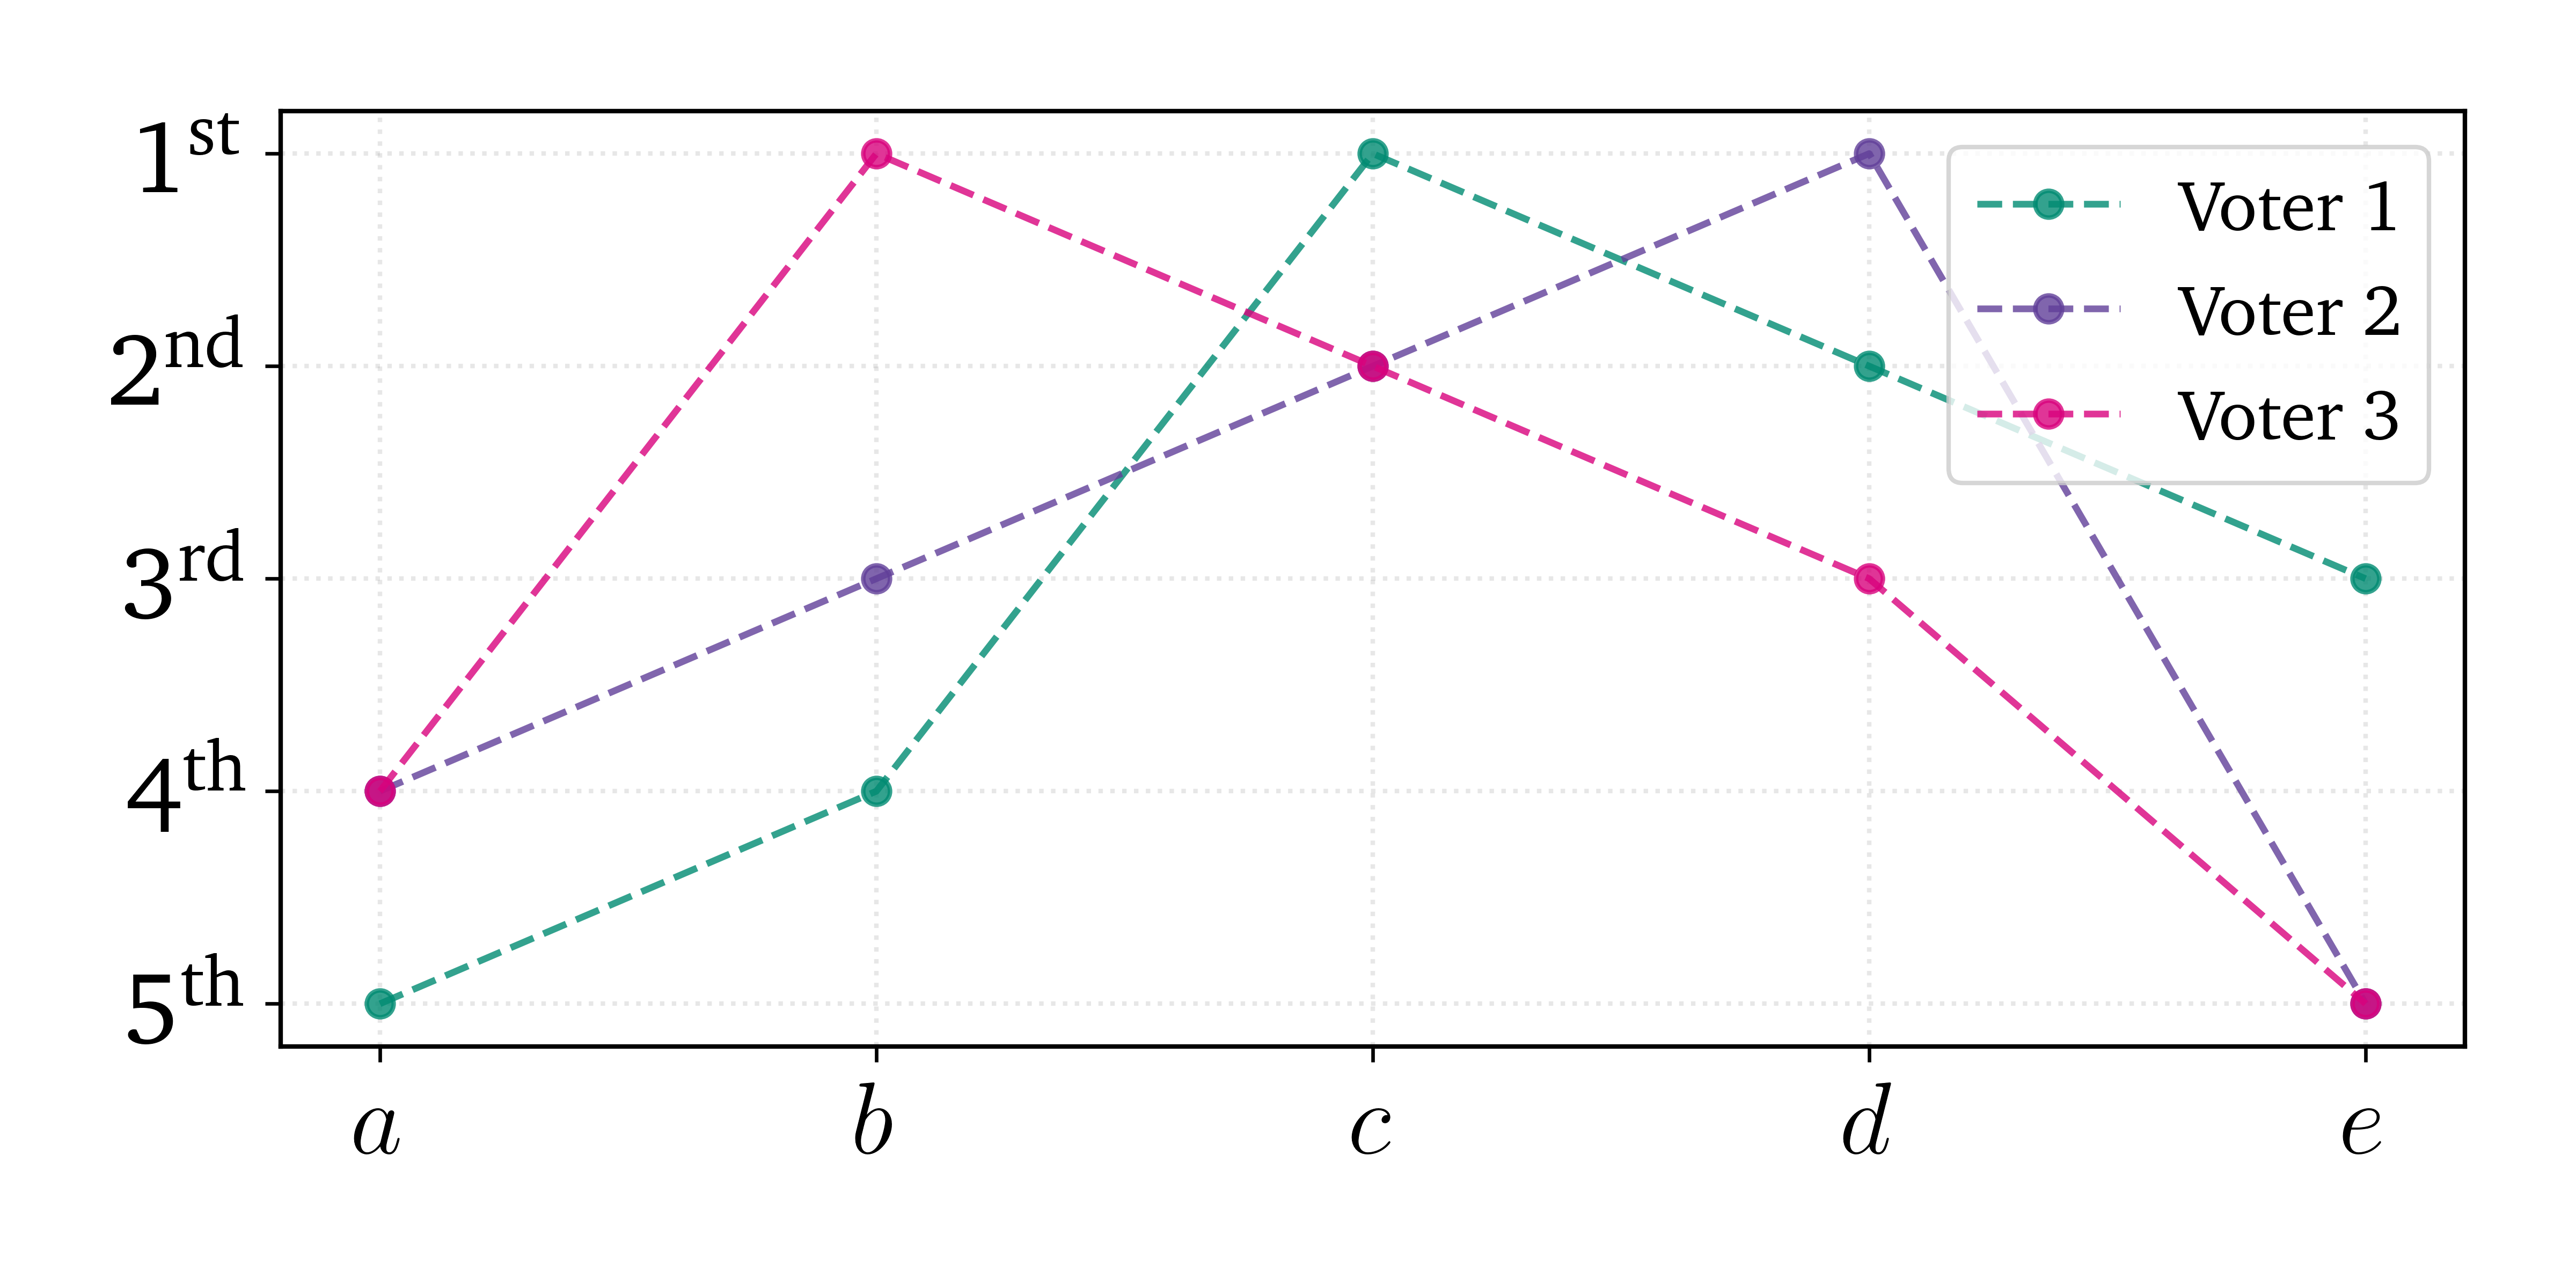
\includegraphics[width=\textwidth]{Figures/single_peak_vis.png}
		\caption{Single-peaked profile visualization}\label{fig:singlepeaked_vis}
	\end{subfigure}
	\caption{An election with three voters and five candidates. Each voter has a unique peak, and the profile is single-peaked with respect to a shared axis.}
	\label{fig:singlepeaked_full}
\end{figure}
\begin{definition}{Single-peaked Profiles}{single-peaked}
	A profile $\strictProfile$ is single-peaked, if given some ordering
	$\orderalt$ over the candidates, it holds that for all voters $i$, and
	all $a, b, c \in \alternatives$, if $a \orderalt b \orderalt c$, then
	at most $a \pref_i b$ or $c \pref_i b$, but never both.
\end{definition}

This thesis will now focus on measures to ``increase'' single-peakedness of profile.



